% Options for packages loaded elsewhere
\PassOptionsToPackage{unicode}{hyperref}
\PassOptionsToPackage{hyphens}{url}
\PassOptionsToPackage{dvipsnames,svgnames*,x11names*}{xcolor}
%
\documentclass[
]{article}
\usepackage{lmodern}
\usepackage{amssymb,amsmath}
\usepackage{ifxetex,ifluatex}
\ifnum 0\ifxetex 1\fi\ifluatex 1\fi=0 % if pdftex
  \usepackage[T1]{fontenc}
  \usepackage[utf8]{inputenc}
  \usepackage{textcomp} % provide euro and other symbols
\else % if luatex or xetex
  \usepackage{unicode-math}
  \defaultfontfeatures{Scale=MatchLowercase}
  \defaultfontfeatures[\rmfamily]{Ligatures=TeX,Scale=1}
\fi
% Use upquote if available, for straight quotes in verbatim environments
\IfFileExists{upquote.sty}{\usepackage{upquote}}{}
\IfFileExists{microtype.sty}{% use microtype if available
  \usepackage[]{microtype}
  \UseMicrotypeSet[protrusion]{basicmath} % disable protrusion for tt fonts
}{}
\makeatletter
\@ifundefined{KOMAClassName}{% if non-KOMA class
  \IfFileExists{parskip.sty}{%
    \usepackage{parskip}
  }{% else
    \setlength{\parindent}{0pt}
    \setlength{\parskip}{6pt plus 2pt minus 1pt}}
}{% if KOMA class
  \KOMAoptions{parskip=half}}
\makeatother
\usepackage{xcolor}
\IfFileExists{xurl.sty}{\usepackage{xurl}}{} % add URL line breaks if available
\IfFileExists{bookmark.sty}{\usepackage{bookmark}}{\usepackage{hyperref}}
\hypersetup{
  pdftitle={Data Story: Narrative Basics},
  pdfauthor={Zach del Rosario},
  colorlinks=true,
  linkcolor=Maroon,
  filecolor=Maroon,
  citecolor=Blue,
  urlcolor=cyan,
  pdfcreator={LaTeX via pandoc}}
\urlstyle{same} % disable monospaced font for URLs
\usepackage[margin=1in]{geometry}
\usepackage{longtable,booktabs}
% Correct order of tables after \paragraph or \subparagraph
\usepackage{etoolbox}
\makeatletter
\patchcmd\longtable{\par}{\if@noskipsec\mbox{}\fi\par}{}{}
\makeatother
% Allow footnotes in longtable head/foot
\IfFileExists{footnotehyper.sty}{\usepackage{footnotehyper}}{\usepackage{footnote}}
\makesavenoteenv{longtable}
\usepackage{graphicx,grffile}
\makeatletter
\def\maxwidth{\ifdim\Gin@nat@width>\linewidth\linewidth\else\Gin@nat@width\fi}
\def\maxheight{\ifdim\Gin@nat@height>\textheight\textheight\else\Gin@nat@height\fi}
\makeatother
% Scale images if necessary, so that they will not overflow the page
% margins by default, and it is still possible to overwrite the defaults
% using explicit options in \includegraphics[width, height, ...]{}
\setkeys{Gin}{width=\maxwidth,height=\maxheight,keepaspectratio}
% Set default figure placement to htbp
\makeatletter
\def\fps@figure{htbp}
\makeatother
\setlength{\emergencystretch}{3em} % prevent overfull lines
\providecommand{\tightlist}{%
  \setlength{\itemsep}{0pt}\setlength{\parskip}{0pt}}
\setcounter{secnumdepth}{-\maxdimen} % remove section numbering

\title{Data Story: Narrative Basics}
\author{Zach del Rosario}
\date{2020-05-15}

\begin{document}
\maketitle

\emph{Purpose}: The point of data science is not to gather a random pile
of facts; it's to \emph{do something} with those facts. One of our key
goals in data science is to help drive decisions and action---we
accomplish this by communicating our \emph{data story}. Since story is
fundamentally an exercise in narrative, we'll start our data story
training with some narrative basics.

\emph{Reading}: \href{https://www.youtube.com/watch?v=ERB7ITvabA4}{Randy
Olson's TED Talk}, introducing the \emph{And, But, Therefore} (ABT)
framework. \emph{Reading Time}: \textasciitilde{} 10 minutes

\emph{Lesson Plan}: Ensure all students submit their narrative spectrum
classifications and justification through the Google Form. Set aside a
full-class meeting to discuss the student results. Visualize the
results, and see what (if any) consensus the class came to. Ask a few
students who classified the graphs differently to share their
perspective. After gathering student input, offer your own perspective
on the graph. Repeat for each example.

Make sure to emphasize that different people will read graphs
differently; we don't have \emph{complete control} over the narrative
when presenting a graph. But the simpler and more focused our graph, the
better control we have over the narrative experienced. (TODO: Future
exercises/activities should emphasize this!)

\hypertarget{exposition}{%
\subsection{Exposition}\label{exposition}}

Scientist-turned-storyteller Randy Olson{[}1{]} introduced the
\emph{narrative spectrum}. Three points along the spectrum are listed
below:

\begin{longtable}[]{@{}lll@{}}
\toprule
TLA & Framework & Narrative Spectrum\tabularnewline
\midrule
\endhead
AAA & And, And, And & Non-narrative\tabularnewline
ABT & And, But, Therefore & Just right!\tabularnewline
DHY & Despite, However, Yet & Overly-narrative\tabularnewline
\bottomrule
\end{longtable}

The narrative spectrum runs from non-narrative: introducing no conflict
or tension, to overly-narrative: introducing too many conflicting ideas.
Olson observed that the middle of the narrative spectrum is just the
right amount of narrative content. The extreme points tend to be boring:

\begin{itemize}
\tightlist
\item
  A child may tell a story like ``We went to the store, AND the man had
  a hat, AND I lost a shoe, AND we went home.'' This story lacks any
  narrative content: no part of the story relates to any other part, so
  no conflict or drama can arise. (AAA)
\item
  An extremely learned professor may tell a story like ``Kolmogorov
  proposed a 5/3 power law. HOWEVER Smith found 3/8 power law behavior.
  YET Chandrasekhar discovered a 2/3 power law\ldots.'' This story
  swings in the opposite direction; there is \emph{too much conflict},
  and most listeners will be totally lost. This is the proverbial
  \emph{random pile of facts} we need to avoid when communicating. (DHY)
\end{itemize}

Using the ABT framework can help us get started with framing a story.
For example:

``Data science is the use of computation and statistics to learn from
data AND we want to use data science to help people make decisions BUT a
random pile of facts will lose our audience THEREFORE we will study
narrative to help tell our data story.''

The \textbf{AND} part of the framework is our \emph{exposition}; every
story needs some setup. The \textbf{BUT} part introduces some
conflict---in a hollywood story this could be a murder, but in science
it could be an unexplained phenomenon. \textbf{THEREFORE} is where we
pay off the exposition and conflict. In our hollywood story its where we
solve the murder. In science its where we learn something about reality,
and pose the next exciting question to investigate.

\emph{Note}: The ABT framework is \textbf{not the only way to tell a
story}. It is a simplified framework to help us get started!

\hypertarget{exercises-judging-narrative-content}{%
\subsection{Exercises: Judging Narrative
Content}\label{exercises-judging-narrative-content}}

Now let's put all that narrative theory to use! We're going to judge a
number of graphs based on their narrative content, placing them at a
point on Olson's narrative spectrum. To do so, we're going to need some
framing for the following exercise:

\textbf{For this exercise}, pretend that you are going to show the
following graphs to a very busy data scientist.

The following graphs are not intended for you to use to discover things.
They are intended to communicate your findings to someone else. Your
data science colleague is smart and competent (she knows what a boxplot
is, understands variability, etc.), but she's also busy. You need to
present a figure that \emph{tells a story} quickly, or she's going to
use her limited time to think about something else.

\textbf{Your task}: Study the following graphs and determine \emph{the
closest point}---AAA, ABT, or DHY---near which the example lies on
narrative spectrum. Keep in mind your intended audience (your colleague)
when judging how much or how little narrative content is present.

\begin{verbatim}
## -- Attaching packages ----------------------------------------- tidyverse 1.3.0 --
\end{verbatim}

\begin{verbatim}
## v ggplot2 3.3.2     v purrr   0.3.4
## v tibble  3.0.1     v dplyr   1.0.0
## v tidyr   1.1.0     v stringr 1.4.0
## v readr   1.3.1     v forcats 0.5.0
\end{verbatim}

\begin{verbatim}
## -- Conflicts -------------------------------------------- tidyverse_conflicts() --
## x dplyr::filter() masks stats::filter()
## x dplyr::lag()    masks stats::lag()
\end{verbatim}

\textbf{q1} Identify the point on the narrative spectrum, and justify
your answer.

\emph{Hint}: Try telling yourself a story based on the graph! This can
be your \textbf{justification} for the narrative spectrum point you
select.

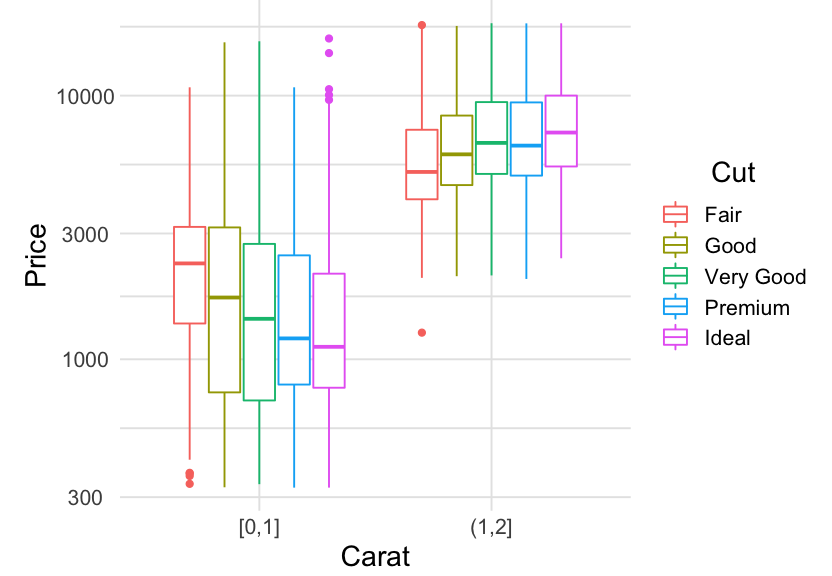
\includegraphics{e-comm01-story-basics_files/figure-latex/q1-vis-1.png}

\textbf{Classify}: AAA, ABT, or DHY? ABT

\textbf{Justify} Write your justification here! At low carat, an
improvement in \texttt{cut} tends to \emph{decrease} \texttt{price}.
However, at a higher carat, an improvement in \texttt{cut} tends to
\emph{increase} \texttt{price}. This graph conveys a small amount of
information, but still manages to introduce some conflict.

\newpage

\textbf{q2} Identify the point on the narrative spectrum, and justify
your answer.

\begin{verbatim}
## `geom_smooth()` using method = 'gam' and formula 'y ~ s(x, bs = "cs")'
\end{verbatim}

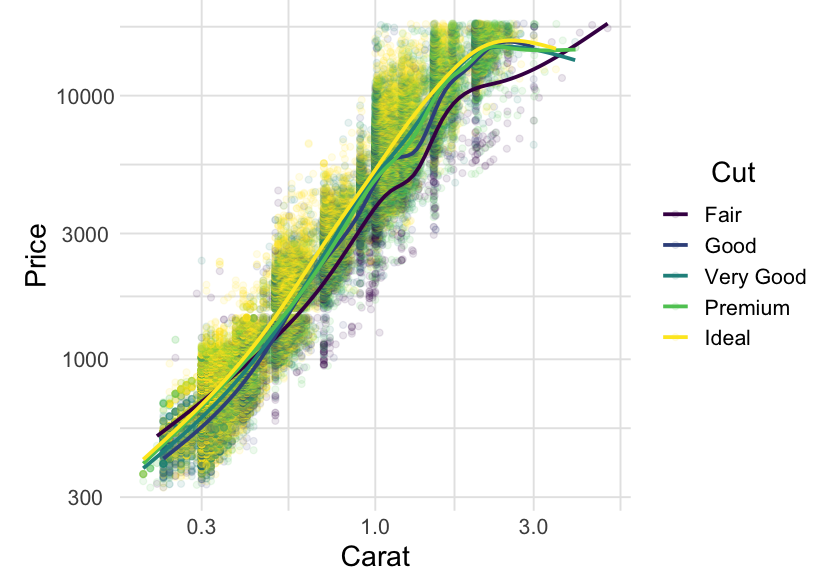
\includegraphics{e-comm01-story-basics_files/figure-latex/q2-vis-1.png}

\textbf{Classify}: AAA, ABT, or DHY? DHY

\textbf{Justify} Write your justification here! Diamonds tend to be
\texttt{price} ordered by their \texttt{cut}. However, at low
\texttt{carat} the \texttt{Fair} diamonds tend to be most pricey. Yet
\texttt{Good}, \texttt{Very\ Good} and \texttt{Premium} diamonds tend to
overlap. There are too many conflicting ideas in this graph to quickly
tell a compelling story.

\newpage

\textbf{q3} Identify the point on the narrative spectrum, and justify
your answer.

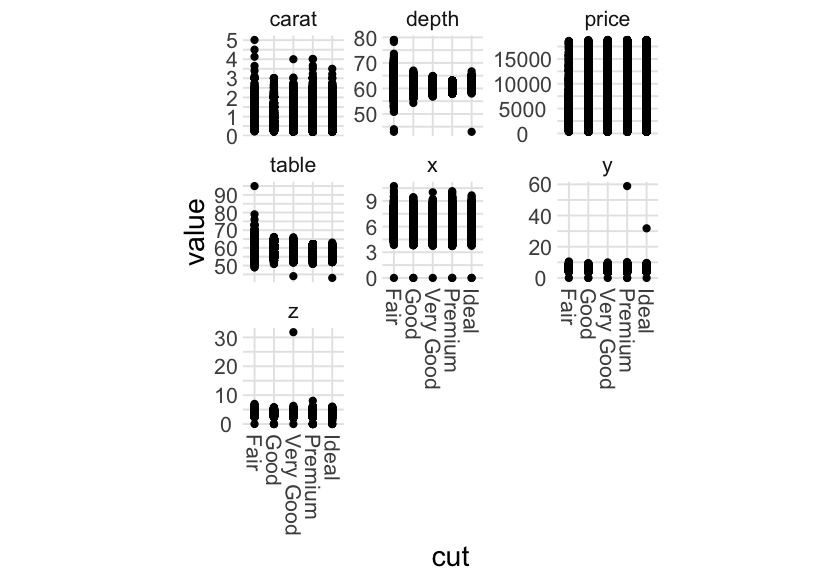
\includegraphics{e-comm01-story-basics_files/figure-latex/q3-vis-1.png}

\textbf{Classify}: AAA, ABT, or DHY? AAA

\textbf{Justify} Write your justification here! The highest
\texttt{carat} diamonds tend to be \texttt{Fair}, and \texttt{Fair}
diamonds tend to vary a lot in \texttt{depth}, and \texttt{price} varies
widely for all \texttt{cut} values, and some diamonds have
\texttt{x,\ y,\ z} values at zero\ldots.

\newpage

\textbf{q4} Turn in all your answers via google forms.
\href{https://forms.gle/kHuT5oufUQA7jRWG8}{Link}

\hypertarget{exit-ticket}{%
\section{Exit Ticket}\label{exit-ticket}}

Once you have completed this exercise, make sure to fill out the
\textbf{exit ticket survey},
\href{https://docs.google.com/forms/d/e/1FAIpQLSeuq2LFIwWcm05e8-JU84A3irdEL7JkXhMq5Xtoalib36LFHw/viewform?usp=pp_url\&entry.693978880=e-comm01-story-basics.Rmd}{linked
here}.

\hypertarget{bibliography}{%
\section{Bibliography}\label{bibliography}}

\begin{itemize}
\tightlist
\item
  {[}1{]} Olson, \href{http://scienceneedsstory.com/}{``Houston, We Have
  a Narrative''} (2015)
\end{itemize}

\end{document}
